\documentclass[12pt,a4paper,twoside,openright]{book}

\usepackage[english]{babel}
\usepackage[utf8]{inputenc}

\usepackage{style/isi_style_lt}

\usepackage{amsmath,amsfonts,amssymb,amsthm}
\usepackage{caption}
\usepackage[usenames]{color}
\usepackage{enumerate}
\usepackage{fancyhdr}
\usepackage{fancyvrb}
\usepackage{float}
\usepackage{graphicx}
\usepackage{indentfirst}
\usepackage{listings}
\usepackage{marvosym}
\usepackage{multicol}
\usepackage{sectsty}
\usepackage{subcaption}
\usepackage{tocloft}
\usepackage[table]{xcolor}
\usepackage{url}
\usepackage{lmodern,textcomp}
\usepackage{multirow}

\AtBeginDocument{%
	\renewcommand{\contentsname}{Table of Contents}
	\renewcommand\tablename{Table}
	\renewcommand\figurename{Figure}
	\renewcommand{\lstlistingname}{Lis}
	\renewcommand{\refname}{Ref}
}

\definecolor{dkgreen}{rgb}{0,0.6,0}
\definecolor{gray}{rgb}{0.5,0.5,0.5}
\definecolor{mauve}{rgb}{0.58,0,0.82}

\lstset{
  frame=single,
  captionpos=b,
  language=Java,
  aboveskip=3mm,
  belowskip=3mm,
  showstringspaces=false,
  columns=flexible,
  basicstyle={\small\ttfamily},
  numbers=none,
  numberstyle=\tiny\color{gray},
  keywordstyle=\color{blue},
  commentstyle=\color{dkgreen},
  stringstyle=\color{mauve},
  breaklines=true,
  breakatwhitespace=true,
  tabsize=3
}

\makeatletter
\def\cleardoublepage{
	\clearpage\if@twoside \ifodd\c@page\else
	\hbox{}
	\thispagestyle{empty}
	\newpage
	\if@twocolumn\hbox{}\newpage\fi\fi\fi
}

\makeatother

\setlength{\textwidth}{14cm}
\setlength{\textheight}{21cm}
\setlength{\footskip}{3cm}

\setlength{\hoffset}{0pt}
\setlength{\voffset}{0pt}

\setlength{\oddsidemargin}{1cm}
\setlength{\evensidemargin}{1cm}

\universita{Alma Mater Studiorum -- University of Bologna}

\campus{Campus of Cesena}

\scuola{Engineering and Architecture Faculty}

\corsodilaurea{Master's Degree in Engineering and IT}

\titolo{Robot Exploration}

\materia{Intelligent Robotic Systems}

\laureando{Gabriele Guerrini}

\annoaccademico{2019 -- 2020}

\makeindex

\begin{document}

\frontmatter 

\maketitle

\tableofcontents

\mainmatter

\pagestyle{fancy} 
\fancyhead[LE,RO]{\thepage}
\fancyfoot{}
\raggedbottom
	
\chapter{Project goal}

\chapter{State of the art}

An overall of four different well-known tasks can be detected in the problem, namely:

\begin{itemize}

  \item \textbf{Arena exploration}: the robots must explore the arena to find the landmarks.
  \item \textbf{Clustering}: the robots must create cluster near any landmark so it can be considered explored.
  \item \textbf{Phototaxis}: used to allow the robots to easily come back to the base.
  \item \textbf{Obstacle avoidance}: general behaviour to be executed to prevent any collision (between robots as well as between robots and obstacles/walls).

\end{itemize}

\noindent
It follows a brief description of the state of the art for each task.

\section{Arena exploration}
The exploration of the area is a well-known task in the literature, and lots of algorithms and methodologies have been studied. However, when talking about swarm robotics, the main adopted method is the \textit{random walk} approach. This is mainly due to the usage of off-the-shelf robots that own limited individual abilities (low processing power, local sensing etc.). Nevertheless, the usage of a swarm of robots for exploration tasks is still widely applied thanks to the advantages it entails respect to the usage of a single robot (flexibility, robustness, scalability).

\bigskip
There are few different common sense implementations of a random walk task \cite{rw-summary}, namely:

\begin{itemize}

  \item {Brownian motion}
  
  \item {Lèvy Flight}
  
  \item {Lèvy Taxis}

  \item {Correlated radom walk}

  \item{Ballistic motion}  
\end{itemize}
 
The main idea is to randomly choose a direction and go straight till a new one is selected.

\noindent
All the aforementioned models share the same underlying mathematical model, and the different tuning of the parameters provides different behaviours and exploration capabilities. Only one exception can be identified, that is the ballistic motion, where the two parameters \textit{step length} ($\mu$) and \textit{turning angle} ($\rho$) are not provided and/or limited. 

\bigskip
Further from the above basic approaches, new solution have been probed to overcome the limits they impose. Indeed, there are two main problem that emerge, that is:

\begin{itemize}

  \item Execution of repeated exploration of the same point.
  \item Exploration does not scale with arena widening. Ineed, just zona near the starting position will be quite well explored.
 
\end{itemize}

New approaches have been studied to overcome the aboe issues. The example reported in \cite{rw-improved} improves the random walk by considering relative distribution of robots among the arena so that each zone can be equally explored by a even quantity of robots.  

\bigskip
Once the robots are spread over the arena, different algorithm can be applied to map it (e.g., \textit{GMapping} that produces a two-dimensional occupancy grid of the environment). 

\section{Clustering}

Clustering is one of the main tasks identified in most of the proposed taxonomies for swarm robotics. The goal is to gather objects (the robot themselves or tokens to be moved) in one or more points of the arena. The task can be used for multiple purposes: foraging activity (group food supplies), divide robots upon classes that execute different tasks, etc..

\noindent
All the proposed clustering algorithms create different solutions upon one of three common approaches \cite{clustering-summary}, that is:

\begin{itemize}

  \item Force-oriented solutions (similar to motor schema principles).
  \item Probabilistic approach by using non-deterministic transition among states and tasks. Indeed, as stated in \cite{clustering-randomness} \cite{clustering-data}, randomness resulted to be a crucial aspect for emerging behaviours in swarm robotics in general. 
  \item Artificial evolution through genetic algorithms. 

\end{itemize}

Independently from the ad hoc approach, the main idea is to apply \textit{swarm intelligence} principles to guide robots behaviour, and so to create a result inspired to various animal species (insects, birds, fishes) or natural laws (e.g., the settling process of liquids of different densities, \cite{clustering-natural}). 

\noindent
Beyond this, few more articulated experiments have been executed trying to add further capabilities to robots (e.g., \textit{spatial awareness} and exchange of \textit{virtual tokens}, \cite{clustering-awareness}).

\noindent
In the end, notice that swarm intelligence principles can be applied to other domains as well. Indeed, lots of experiments have been made about the clustering of data (instead of robots) in order to overcome traditional clustering algorithms such as \textit{K-means} by blending swarm intelligence with other domains (e.g., game theory, \cite{clustering-data}). 

\section{Obstacle avoidance}

The obstacle avoidance task has been widely studied, and so few different algorithms have been proposed. 
The input values can be retrieved with distance sensors (e.g., sonar, proximity sensors) and/or visual sensors. In this case, we are going to focus on techniques that exploit the first ones solely.

\smallskip
The most known technique is the \textit{Artificial Potential Field (APF)} that is based upon the motor schema idea by creating two potential fields: the first is attractive and generated by the goal point so that the robot can aim toward it, the second one is repulsive and it is generated from obstacles. Obviously, even though this method suffers all the issues of the motor schema approach such as local minima, it finds shorter paths than other well-know algorithm such as the \text{Bug} one \cite{obstacle-summary} \cite{obstacle-summary-2}.

\noindent
Other solutions, even though rely on the same underlying mathematical model, contemplate different types of potential fields: tangential fields to circumnavigate obstacles, Gaussian potential fields \cite{obstacle-gaussian}.

\noindent
In addition, we notice the \textit{Vector Field Histogram} algorithm that produces a vector force as output (length, angle), but differently from others it exploits peculiar tools as histograms to represent the distribution of obstacles around the robot. The algorithm provides for three stages so that the initial 2D histogram is collapsed to a polar one.  

\noindent
Moreover, as well as the classical approaches, novel solutions have been explored by combining genetic algorithms and neural networks (as reported in \cite{obstacle-NN}).

\noindent
In the end, complete navigation with obstacle avoidance have been experimented by using the \textit{Particle Swarm Optimization} algorithm \cite{obstacle-summary-2}.





\chapter{Solution development}

\section{Behaviour design}

The behavior of each robot is modeled using a non-deterministic finite state automata (\textit{NFA})(see figure \ref{fig:NFA}). Such an architecture has been chosen for the robot since its behavior is not trivial and more tasks must be executed at different times. By using a FSA, it is easy to explicitly express activities, conditions and non-deterministic transitions. Moreover, each state can be developed as a separated module, and the most suitable solution can be implemented case by case.

\noindent
The robot starts in the ``resting'' state. A non-deterministic transition makes the robot leave the base and start the exploration with a probability $P1$. 

\noindent
When exploring, the robot looks for any close landmark and, if it is the case, it joins the cluster around such landmark with a probability $P2$ and enters in ``waiting for cluster to complete" state. Moreover, the robot may quit the exploration task at any moment and return to the base with a probability $P3$. In the latter casuistry, the robot enters in the ``returning to base" state.

\noindent
When a cluster is completed by reaching the required number of robots $N$, the robot enters in the ``reconnaissance'' state. Such a state conceptually correspond to the phase during which the robots in the cluster should explore the area near the landmark. Such a task is not executed in this project for simplicity, but few different algorithms have been created to let a set of robots to explore and map a given area.

\noindent
The robot ends the reconnaissance task after $t_1$ seconds, and it returns to the base.

\noindent
When returning to the base, the robot executes a phototaxis task. The robot enters in the ``resting'' state once it is detected that it successfully returned to the base. 

\noindent
In the end, the robot may leave the cluster before it is completed with a probability $P4$. In this case, it enters in the ``biased exploration" state, that is a state where the robot executes the regular exploration tasks
but with inhibited stimuli from landmarks. After $t_2$ seconds it returns in the normal exploration behaviour. Such a intermediate state is required so that the robot may step away from the landmark (otherwise, even though it is a probabilistic transition, it would join the cluster again in most of the cases). TODO: required?  

\begin{figure}[H]
\centering
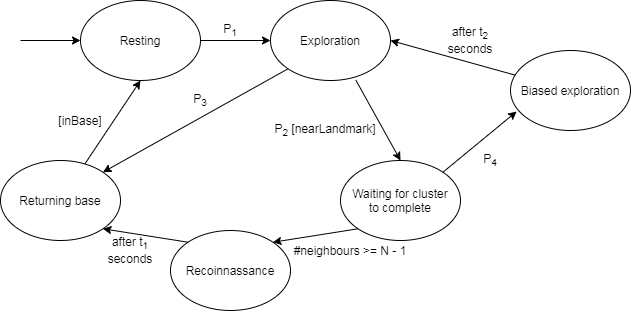
\includegraphics[width=\linewidth]{images/NFA.png}
\caption{\textit{NFA representing the behaviour of the robot. $P_i$ represent a non-deterministic transition that happens with such probability.}}
\label{fig:NFA}
\end{figure}

The implementation of the FSA is executed by using a ``states`` table to store the code be executed in each state. The variable ``current\_state'' represents the current active state, while transition are executed by checking simple``if-then-else'' conditions.

\noindent
In the end, a variable ``t'' stores the time spent by the robot in the current state.

\subsection{Motor schema design}

When a state requires motion, its design has been developed using a motor schema approach and, once the total force suffered by the robot has been calculated, the following formula is used to switch from the translational-angular model to differential one (i.e., find the velocity of each wheel out from the direction and length of the total suffered force):    

\begin{equation}
\begin{bmatrix} 
v_l \\
v_r
\end{bmatrix}
=
\begin{bmatrix} 
1 & -L/2 \\
1 & L/2
\end{bmatrix}
\begin{bmatrix} 
v \\
\omega
\end{bmatrix}
\tag{3.0}\label{eq:3.0}
\end{equation}

\noindent
where:

\smallskip
\noindent
$v_l$ = velocity of the left wheel

\noindent
$v_r$ = velocity of the right wheel

\noindent
$L$ = distance between the two wheels

\noindent
$v$ = translational velocity

\noindent
$\omega$ = angular velocity

\section{Resting}

The robot just checks if a transition to the exploration state should occur, and so no particular architectural style has been adopted for this module. The following function has been used to model the probability:

\begin{equation}
    p = tanh((t - Shift) / Patience) + 1 \tag{3.1}\label{eq:3.1}
\end{equation}

\noindent
The idea is to create a probability that is directly proportional to the time spent in the current state using a non linear relation. Moreover, the probability should grow very slowly at the beginning so that the robot will remain in the resting state for a while. 

\noindent
The function $tanh(x)$ is the basic function used to represent such relation\footnote{A reasonable alternative would be the exponential function, but it requires the tuning of few parameters so that the ``tail'' of the function take reasonable values} (figure \ref{fig:tanh}\footnote{The figure illustrates the regular \textit{tanh} function instead of the one exposed in formula \ref{eq:3.1} since the latter one, despite having a ``similar shape'', can hardly be graphically shown.}). The $Shift$ value is constant (500) so we can take the slice of the function having up concavity while dealing with positive time values. The $Patience$ value is a parameter used to tone all values down. In the end, the $+1$ factor let the function have positive values.  

\noindent
Table \ref{tab:f-values} reports few reference values of the function.

\begin{table}[H]
\centering
\begin{tabular}{| c | c |}

\hline
t & p \\
\hline
 0  & 0.013 \\
 10 & 0.015 \\
 50 & 0.022 \\
100 & 0.036 \\
500 & 1 \\
\hline

\end{tabular}
\caption{\label{tab:f-values}\textit{Few example values of the function used to model dependency with elapsed time using a non linear relation.}}
\end{table}

\begin{figure}[H]
\centering
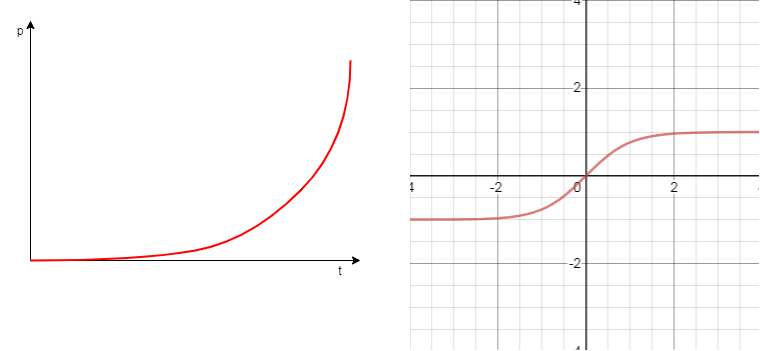
\includegraphics[width=8cm, keepaspectratio]{images/tanh.png}
\caption{\textit{Graph of the tanh function in range [-4;4].}}
\label{fig:tanh}
\end{figure}

\section{Exploration}

The robot executes a ballistic motion. A single potential field is created since the obstacle avoidance feature is implicitly given from the random walk itself. The direction of such potential field is randomly chosen each time an obstacle is detected, while its strength is given by a constant value ``CRUISE\_VELOCITY''. 

\smallskip
When exploring, the robot has a fixed probability to quit such task. Such parameter has been tuned with a very low vale (0.001) in order to avoid too much segmented behaviours where the robots keep on fluctuating just between the two states of ``exploration'' and ``returning to base''.  

\section{Clustering}

A robot may join/create a cluster when close to a landmark with a probability described by the following function:

\begin{equation}
    p =  \frac{(tanh((t - Shift) / Patience) + 1) * tanh(n / NeighborInfluenceLimiter)}{(NeighborInfluenceLimiter * PatienceEnhancer)} \tag{3.2}\label{eq:3.2}
\end{equation}

The probability is proportional to number of robots already in the cluster ($n$) and to the time spent exploring ($t$) both. The same formula in \ref{eq:3.1} has been used the time dependence term. 
The parameter $NeighborInfluenceLimiter$, as the name hints, limits the influence of number of neighbors in the final result.

\noindent
The denominator is a normalization term so reasonable values can be obtained, and it can be tuned by the parameter $PatienceEnhancer$ that makes the robot wait longer as it is increased.

\noindent
Figure \ref{fig:cluster-join} reports the graph of the function in formula \ref{eq:3.2}.

\begin{figure}[H]
\centering
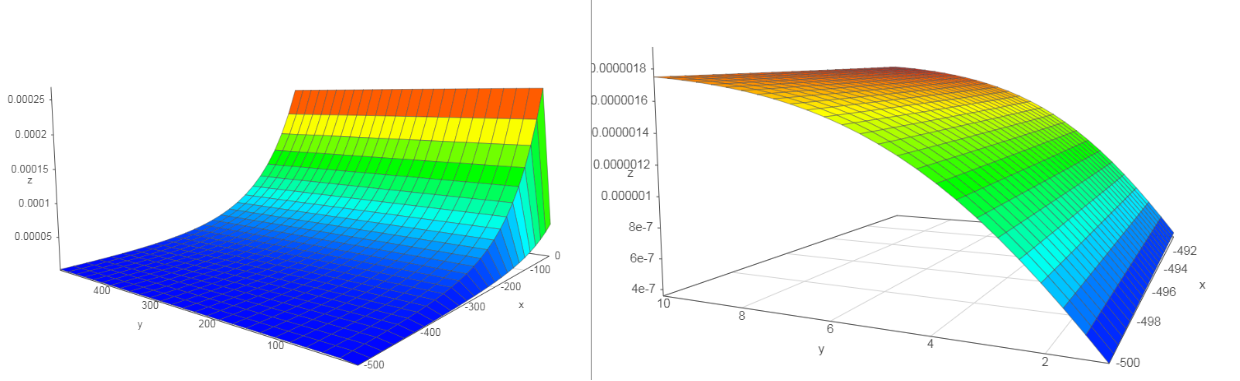
\includegraphics[width=\linewidth]{images/cluster_join.png}
\caption{\textit{x-axis = time, y-axis = number of neighbors, z-axis = probability. Graph of the plot in domain [-500;0], [1;500]  showing the total trend of the function (left) so the time relation can be shown well. On the right, a zoom in in range [-500; -492], [1:10] is executed to show the dependence upon neighbors (indeed, the number of robots in the cluster will never be about the previous order of magnitude ($10^2$) , and so low values, that cannot be appreciated in the left graph, are the the ones of interest.}}
\label{fig:cluster-join}
\end{figure}

Similarly, the probability for a robot to leave a cluster before it is completed is modeled using the following function:

\begin{equation}
    p =  \frac{(tanh((t - Shift) / Patience) + 1) / tanh(n / NeighborInfluenceLimiter)}{(NeighborInfluenceLimiter * PatienceEnhancer)} \tag{3.3}\label{eq:3.3}
\end{equation}

Formula \ref{eq:3.2} and \ref{eq:3.3} are exactly the same function except for a sign (division instead of multiplication of the two terms that model relation with time and number of neighbors). Indeed, the robot increases its probability to leave as time passes (direct proportionality) but, at the same time, its probability to leave is decreased as the number of perceived neighbors increases (inverse proportionality)(the more robots, the more probability to complete the cluster soon is the underlying reason that may lay under such behavior). 

\noindent
Figure \ref{fig:cluster-leave} reports the graph of the function in \ref{eq:3.3}.

\begin{figure}[H]
\centering
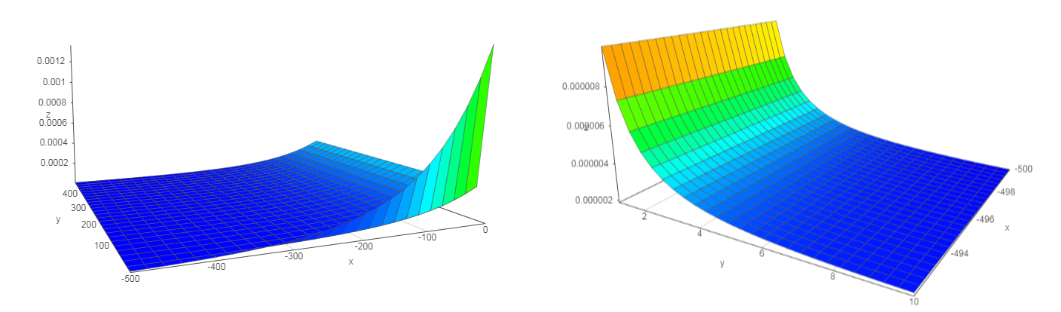
\includegraphics[width=\linewidth]{images/cluster_leave.png}
\caption{\textit{Similal reasonings of figure \ref{fig:cluster-join}. The probability slowly increases as time passes (x-axis) and rapridly decreases as numbe of neighbors increases (y-axis).}}
\label{fig:cluster-leave}
\end{figure}

\section{Returning to base}

This state must mixes phototaxis and obstacle avoidance, and so a motor schema approach has been used to easily blend such two tasks.

\smallskip
The phototaxis capability is created by using an attractive potential field produced by the light source. Hence, the resulting force, whose direction guides to robot toward the light source, has a value inversely proportional to the perceived light.

\smallskip
The obstacle avoidance capability is created by using a tangential field around any obstacle so the robot can circumnavigate boxes or other robots. By exploiting proximity sensors, a perpendicular force is created($\pi/2$ from the sensor orientation, and proportional to the proximity). A possible issue is given from the boundary walls that may create local minima in some rare cases. However, such problem may be fixed by introducing a third potential field: a perpendicular one coming from the walls. Moreover, when travelling to base, the robot should not slip into any wall in most of the cases, and so the issue is not of primary importance for the time being.
 



\chapter{Performance evaluation}

\bigskip
Few different arena layouts are used by changing the position of the landmarks. We consider three different arrangements by placing the landmarks:

\begin{itemize}

  \item At the four cardinal points
  \item At the four corners of the arena
  \item Aligned on a same side of the arena

\end{itemize}

The three configurations are reported in figure ?. 

\smallskip
For each arena arena, different configurations are probed by tuning the following parameters, namely:

\begin{itemize}

  \item Number of robots: 20, 30, 40
  \item Expected cluster size: 1, 3, 5
  \item Number of obstacles (boxes): 0, 10, 20

\end{itemize}

The system is evaluated by checking how many landmarks are explored as time passes. A simulation is concluded when time reaches a maximum allowed value (3000). For example, if we have the following values:

\begin{center}
[100, 400, 800, 3000]
\end{center}

The first landmark has been explored at time 100, etc. The last one has not been explored during the simulation, and so its value is set to 3000.

\noindent
We define \textit{goodness} a quantitative metric that estimates how well the system behaves so that we can compare different combinations of parameters in a quantitative way. A given time t is associated to the number of landmarks that had already been explored in such time. Hence, starting from the four exploration times, we can model the trend of the system along the simulation using a time series. Figure ? reports a clarifier example.  



Table \ref{tab:perf-table} reports the \textit{minimum guaranteed level of service} (i.e. worst values among all the executed runs) and the goodness of each casuistry.


\begin{table}[H]
\centering
\begin{tabular}{| c c c | c c c c | c |}

\hline
Robots & Cluster size & Obstacles & \multicolumn{4}{ c |}{Time} & Goodness \\
\hline
20 & 1 & 0  & 161& 258& 343& 1081 & 0.84 \\
20 & 1 & 10 & 300& 329& 1705& 1931& 0.64\\
20 & 1 & 20 & 266& 370& 863& 2771& 0.64\\
20 & 3 & 0  & 559& 1231& 2730& 3000& 0.37\\
20 & 3 & 10 & 3000& 3000& 3000& 3000& 0.0\\
20 & 3 & 20 & 3000& 3000& 3000& 3000& 0.0\\
20 & 5 & 0  & 3000& 3000& 3000& 3000& 0.0\\
20 & 5 & 10 & 3000& 3000& 3000& 3000& 0.0\\
20 & 5 & 20 & 3000& 3000& 3000& 3000& 0.0\\
\hline
30 & 1 & 0  & 115& 372& 414& 1032& 0.83\\
30 & 1 & 10 & 234& 418& 548& 2112& 0.72\\
30 & 1 & 20 & 317& 623& 994& 3000& 0.58\\
30 & 3 & 0  & 869& 1165& 2401& 3000& 0.33\\
30 & 3 & 10 & 1449& 1962& 2981& 3000& 0.21\\
30 & 3 & 20 & 1461& 2667& 2990& 3000& 0.15\\
30 & 5 & 0  & 3000& 3000& 3000& 3000& 0.0\\
30 & 5 & 10 & 3000& 3000& 3000& 3000& 0.0\\
30 & 5 & 20 & 3000& 3000& 3000& 3000& 0.0\\
\hline
40 & 1 & 0  & 175& 236& 367& 862& 0.86\\
40 & 1 & 10 & 268& 410& 420& 1022& 0.82\\
40 & 1 & 20 & 307& 580& 1018& 2069& 0.66\\
40 & 3 & 0  & 833& 834& 970& 2566& 0.53\\
40 & 3 & 10 & 1542& 1633& 2394& 2453& 0.33\\
40 & 3 & 20 & 1534& 2815& 3000& 3000& 0.13\\
40 & 5 & 0  & 3000& 3000& 3000& 3000& 0.0\\
40 & 5 & 10 & 3000& 3000& 3000& 3000& 0.0\\
40 & 5 & 20 & 3000& 3000& 3000& 3000& 0.0\\
\hline

\end{tabular}
\caption{\label{tab:perf-table}\textit{Evaluation of the system on 27 proposed combinations. For each casuistry, it is reported the moment of exploration of each landmark. Every value is the worst value among the registered ones. Moreover, the goodness of each combination is reported too.}}
\end{table}


\chapter{Conclusions}

The system has been developed by mixing different well-known techniques such as finite state automata and motor schema. Moreover, the most common swarm intelligence principles have been applied too (local sensing realized through multi-channel range and bearing communication, non-deterministic state transitions with positive/negative feedbacks). The realization of few parts has been made by following the state of the art for such tasks by implementing common sense techniques (exploration for swarm robotics through random walk, obstacle avoidance though  well-known potential fields etc.). 

\noindent
In the end, the system has been evaluated upon multiple configuration of the arena and controller both by changing parameters such as the position of the landmarks, the expected cluster size and number of obstacles. It emerged that the position of landmarks and obstacles is a key factor, while the number of robot is decisive for emerging clustering behaviour.

\bigskip
Further developments may include the implementation of any different exploration strategy aside form the ballistic motion and a refinement of the modules based upon the motor schema approach by inserting a further potential field so walls of the arena are considered too. Moreover, a complete testing of the system on multiple different arenas and controller configurations may be executed so that enough data is available to apply any statistical test (or tuning strategy based on it such as the \textit{F-race} algorithm).      
	
\backmatter	

\begin{thebibliography}{99}

\bibitem{rw-summary}
\url{https://link.springer.com/chapter/10.1007/978-3-030-25332-5_19}

\bibitem{rw-improved}
\url{https://www.hindawi.com/journals/jr/2019/6914212/}

\bibitem{obstacle-NN}
\url{http://anderslyhnechristensen.com/pubs/alchristensen_alifex_holeavoidanceandphototaxis_2006.pdf}

\end{thebibliography}






\end{document}